\section{Pol- Nullstellendiagramm}
\subsection{Stabilitätsbedingungen}
\begin{tabular}{ll}
	stabil & alle Polstellen in der linken Halbebene\\
	grenzstabil & alle Polstellen in der linken Halbebene und/oder auf der
	imaginären Achse\\
	instabil & mindestens eine Polstelle in der rechten Halbebene
\end{tabular}\\

\subsection{PN-Digaramm aus $u(t)$}
Beispiel:
$u(t)=20Ve^{\frac{-t}{50ms}}-15V\cos(1000s^{-1}t+\varphi_{11})+12Ve^{4s^{-1}t}\sin(500s^{-1}t+\varphi_{12})$\\
Polstellen bei: \\
\begin{align}
	20Ve^{\frac{-t}{50ms}} = 20Ve^{-20s^{-1}t} &\rightarrow \text{Pol bei }
	-20s^{-1}\nonumber\\
	-15V\cos(1000s^{-1}t+\varphi_{11}) &\rightarrow \text{Pol bei }
	0\pm1000s^{-1}\nonumber\\
	12Ve^{4s^{-1}t}\sin(500s^{-1}t+\varphi_{12}) &\rightarrow \text{Pol bei } (4\pm
	j500)s^{-1}\nonumber
\end{align}
\usetikzlibrary{shapes}

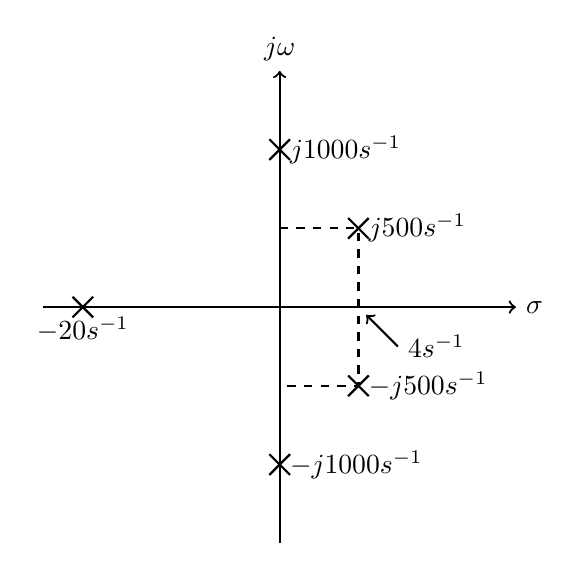
\begin{tikzpicture}[thick]
	\draw [->] (-3,0) -- (3,0);
	\node at (3,0) [anchor=west] {$\sigma$};
	\draw [->] (0,-3) -- (0,3);
	\node at (0,3) [anchor=south] {$j\omega$};
	\draw [dashed] (0,1) -- (1,1) -- (1,-1) -- (0,-1);
	\draw (-2.5,0) node[shape aspect=1,cross out,draw] {};
	\node at (-2.5,0) [anchor=north] {$-20s^{-1}$};
	\draw (0,2) node[shape aspect=1,cross out,draw] {};
	\node at (0,2) [anchor=west] {$j1000s^{-1}$};
	\draw (1,1) node[shape aspect=1,cross out,draw] {};
	\node at (1,1) [anchor=west] {$j500s^{-1}$};
	\draw (1,-1) node[shape aspect=1,cross out,draw] {};
	\node at (1,-1) [anchor=west] {$-j500s^{-1}$};
	\draw (0,-2) node[shape aspect=1,cross out,draw] {};
	\node at (0,-2) [anchor=west] {$-j1000s^{-1}$};
	\draw [->] (1.5,-0.5) -- (1.1,-0.1);
	\node at (1.5,-0.5) [anchor=west] {$4s^{-1}$};
\end{tikzpicture}

\subsection{Frequenzgang $F(j\omega)$ aus PN-Diagramm}
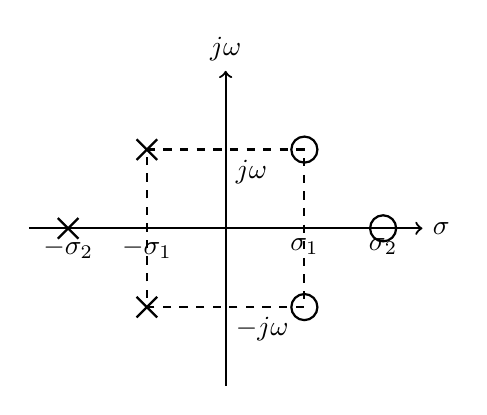
\begin{tikzpicture}[thick]
	\draw [->] (-2.5,0) -- (2.5,0);
	\node at (2.5,0) [anchor=west] {$\sigma$};
	\draw [->] (0,-2) -- (0,2);
	\node at (0,2) [anchor=south] {$j\omega$};
	\draw [dashed] (-1,1) -- (1,1) -- (1,-1) -- (-1,-1) -- (-1,1);

	\draw (-2,0) node[shape aspect=1,cross out,draw] {};
	\draw (-1,1) node[shape aspect=1,cross out,draw] {};
	\draw (-1,-1) node[shape aspect=1,cross out,draw] {};
	
	\draw (1,-1) node[shape aspect=1,circle ,draw] {};
	\draw (1,1) node[shape aspect=1,circle ,draw] {};
	\draw (2,0) node[shape aspect=1,circle ,draw] {};

	\node at (-2,0) [anchor=north] {$-\sigma_2$};
	\node at (-1,0) [anchor=north] {$-\sigma_1$};
	\node at (1,0) [anchor=north] {$\sigma_1$};
	\node at (2,0) [anchor=north] {$\sigma_2$};
	
	\node at (0,1) [anchor=north west] {$j\omega$};
	\node at (0,-1) [anchor=north west] {$-j\omega$};
\end{tikzpicture}\\

$F(j\omega)=K\frac{(j\omega-\sigma_1-j\omega_1)\cdot(j\omega-\sigma_1+j\omega_1)\cdot(j\omega-\sigma_2)}{(j\omega+\sigma_1-j\omega_1)\cdot(j\omega+\sigma_1+j\omega_1)\cdot(j\omega+\sigma_2)}$
